\documentclass{article}
\usepackage{graphicx}
\usepackage{amsmath} 
\usepackage{amssymb}
\begin{document} 
    \begin{titlepage}
    \begin{center}
    \line(1,0){300}\\
    [0.25 in]
    \huge{\bfseries Shihab Muhtasim}\\
    [0.5 cm]
    \textsc{\Large Student ID: 21301610}\\
    \line(1,0){400}\\
    [2 cm]
    \textsc{\LARGE MAT 110}\\
    [0.5 cm]
    \textsc{\LARGE ASSIGNMENT 05}\\
    [0.5 cm]
    \textsc{\LARGE SET 6}\\
    \end{center}
    \end{titlepage}
\begin{newpage}
    \begin{flushright}
    \textsc{Assignment 5}\\
    \textsc{Problem 1}\\
    [1 cm]
    \end{flushright}
\begin{center}
  \textbf{\Large \underline {Ans to the question no 01}}\\
  [0.5 cm]
\end{center}
\Large {Given, \\[3mm]
$-15+12x-6y+y^2=0\\[3mm]
\Rightarrow y^2-6y+3^2=15-12x+9\\[3mm]
\Rightarrow (y-3)^2=-12x+24\\[3mm]
\Rightarrow (y-3)^2=4(-3)(x-2)\\[3mm]
\therefore$ Equation into the standard form of the equation of $ parabola:(y-3)^2=4(-3)(x-2)\\[3mm]$
Comparing this equation with $Y^2=4pX$ we get,\\[3mm]
$Y=y-3,\\[3mm]
4p=12\Rightarrow p=-3,\\[3mm]
X=2-x\\[3mm]$
Vertex:\\[3mm]
$Y=0\\[3mm] \Rightarrow y-3=0 \\[3mm]\Rightarrow y=3\\[3mm]$
Again,\\[3mm]
$X=0 \\[3mm] \Rightarrow x-2=0 \\[3mm] \Rightarrow x=2\\[3mm]
\therefore$ Vertex$(x,y)= (2,3)$\\[5mm]
Focus: \\[3mm]
The focus of the parabola's following $Y^2=4pX$ will be on x axis\\[3mm]
$\therefore Y=0\\[3mm] \Rightarrow y-3=0\\[3mm] \Rightarrow y=3\\[3mm]
And$, $X=p\Rightarrow x-2=-3 \Rightarrow x=-1\\[3mm]
\therefore$ Focus$=(-1,3)\\[3mm]$
Equation of directrix:\\[3mm]
$X+p=0\\[3mm] \Rightarrow x-2-3=0\\[3mm] \Rightarrow x=5\\[3mm]$
Equation of directrix is $x=5$ \\[3mm]}
\end{newpage}
\begin{newpage}
    \begin{flushright}
    \textsc{Assignment 5}\\
    \textsc{Problem 2}\\
    [1 cm]
    \end{flushright}
\begin{center}
  \textbf{\Large \underline {Ans to the question no 02}}\\
  [0.5 cm]
\end{center}
\Large {Given, \\[3mm]
$256+9x^2-160y+16y^2=0\\[3mm]
\Rightarrow 9x^2+16y^2-160y+256=0 \\[3mm]
\Rightarrow 9x^2+16(y^2-10y+25)+256-25\cdot 16=0 \\[3mm]
\Rightarrow 9x^2+16(y-5)^2+144=0 \\[3mm]
\Rightarrow \frac{9x^2}{144}+\frac{16(y-5)^2}{144}=1 \\[3mm]
\Rightarrow \frac{x^2}{4^2}+\frac{(y-5)^2}{3^2}=1 \\[3mm]
\therefore$ Equation into the standard form of the equation of $ ellipse:\frac{x^2}{4^2}+\frac{(y-5)^2}{3^2}=1$\\[3mm]
Comparing this equation with the standard form of equation of ellipse $\frac{(x-h)^2}{a^2}+ \frac{(y-k)^2}{b^2}=1\\[3mm]$
vertex:\\[3mm]
$(h,k)=(0,5)\\[3mm]
a=4, b=3\\[10 cm]$
sketch of the ellipse: \\[3mm]}
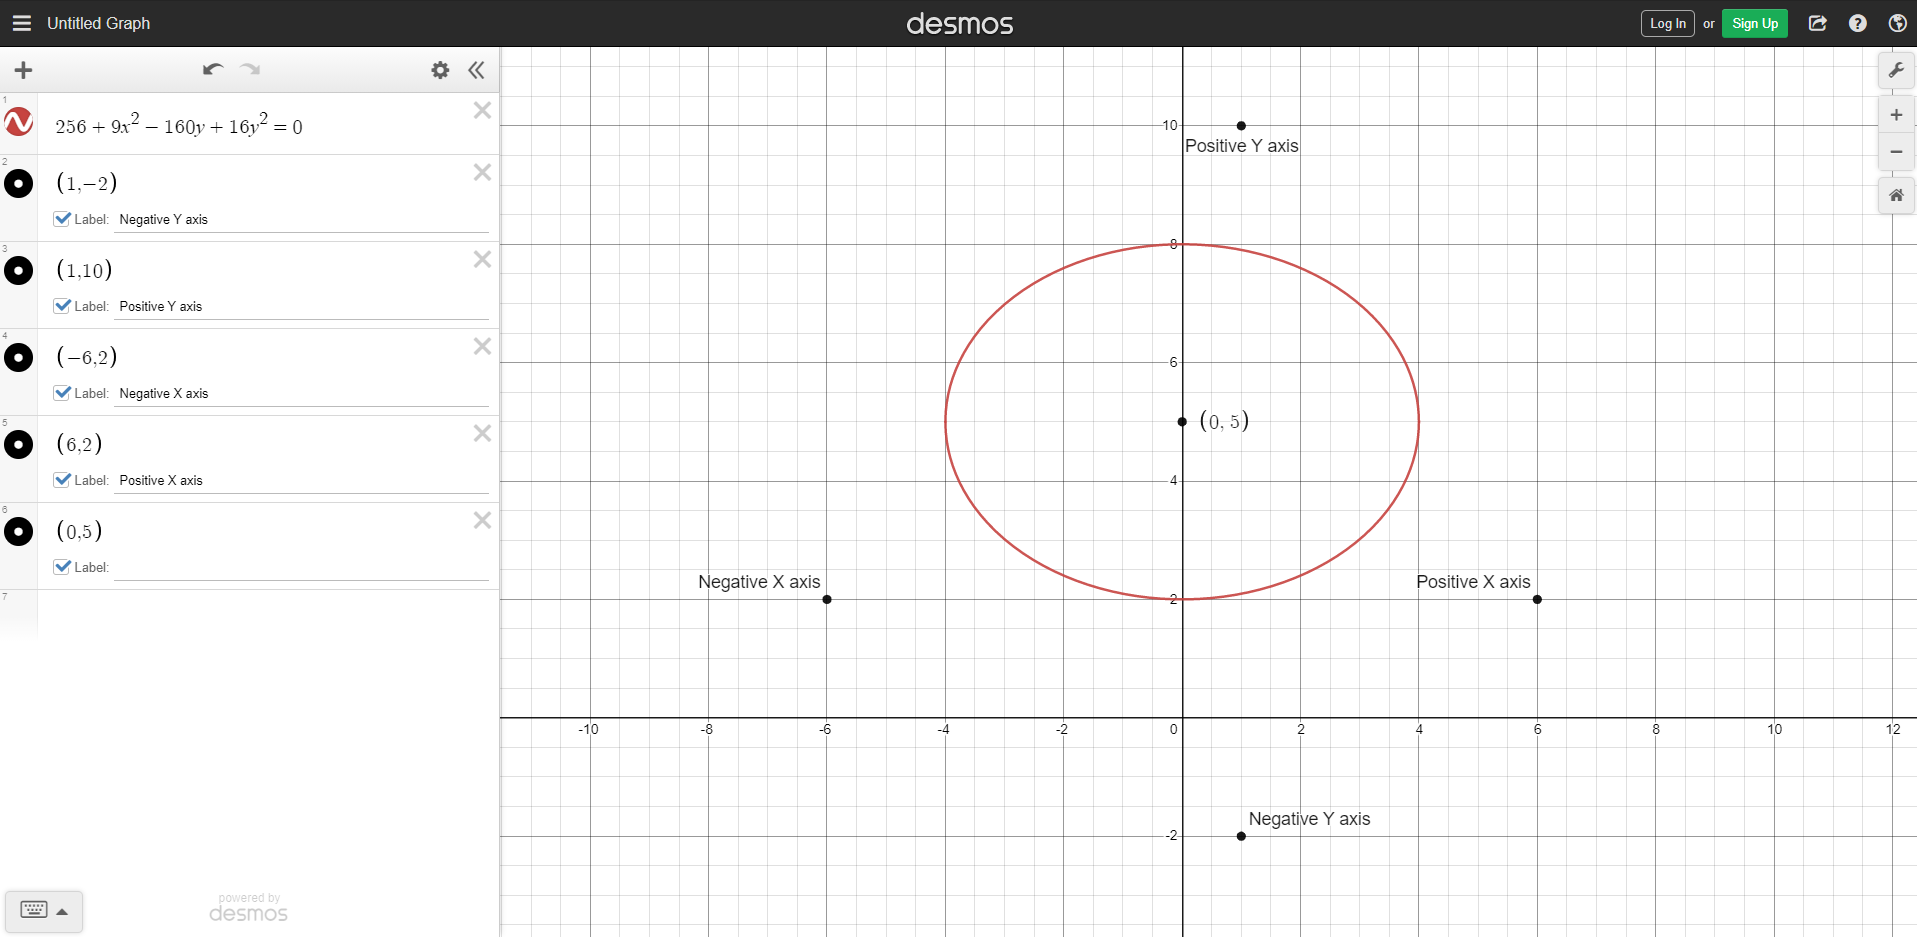
\includegraphics[width=15cm]{sketch question 2}
\end{newpage}
\begin{newpage}
    \begin{flushright}
    \textsc{Assignment 5}\\
    \textsc{Problem 3}\\
    [1 cm]
    \end{flushright}
\begin{center}
  \textbf{\Large \underline {Ans to the question no 03}}\\
  [0.5 cm]
\end{center}
\Large {Given, \\[3mm]
$-24-24x+12x^2-3y^2=0\\[3mm]
\Rightarrow 12(x^2-2x+1)-3y^2-24-12=0 \\[3mm]
\Rightarrow 12(x-1)^2-3y^2=36 \\[3mm]
\Rightarrow \frac{(x-1)^2}{(\sqrt{3})^2}-\frac{y^2}{(2\sqrt{3})^2}=1 \\[3mm]
\therefore$ Equation into the standard form of the equation of  hyperbola:$\frac{(x-1)^2}{(\sqrt{3})^2}-\frac{y^2}{(2\sqrt{3})^2}=1\\[3mm]$
Comparing this equation with the standard form of equation of hyperbola $\frac{(x-h)^2}{a^2}- \frac{(y-k)^2}{b^2}=1,\\[3mm]
a=\sqrt{3},b=2\sqrt{3}\\[3mm]$
Center:$(h,k)=(1,0)\\[3mm]$ 
vertices:\\[3mm]
The vertices of this hyperbola  are on x axis\\[3mm]
$\therefore y=k=0$\\[3mm]
And, $x=h\pm a=1 \pm \sqrt{3}\\[3mm]
\therefore  $ Vertices= $(1+\sqrt{3},0),(1-\sqrt{3},0)$\\[3cm]
Eccentricity:\\[3mm]
$e=\sqrt{1 + \frac{b^2}{a^2} }\\[3mm]
=\sqrt{1+\frac{2\sqrt{3})^2}{(\sqrt{3})^2}}\\[3mm]
=\sqrt{5}\\[3mm]$
Foci:\\[3mm]
$(h \pm ae,k)=(1 \pm \sqrt{3} \cdot \sqrt{5},0)=(1 \pm \sqrt{15} ,0)\\[3mm]
\therefore $ Foci=$(1+\sqrt{15} ,0),(1-\sqrt{15} ,0) \\[3mm]$
Equation of directrices:\\[3mm]
$x-h=\pm \frac{a}{e}\\[3mm]
\Rightarrow x-1=\pm \frac{\sqrt{3}}{\sqrt{5}}\\[3mm]
\Rightarrow x=1 \pm \frac{\sqrt{3}}{\sqrt{5}}\\[3mm]
\Rightarrow x=\frac{5\pm \sqrt{15}}{5}\\[3mm]
\therefore$ Equation of directrices:  $ x=\frac{5 + \sqrt{15}}{5},x=\frac{5 + \sqrt{15}}{5}$\\[3mm]}
\end{newpage}
\begin{newpage}
    \begin{flushright}
    \textsc{Assignment 5}\\
    \textsc{Problem 4}\\
    [1 cm]
    \end{flushright}
\begin{center}
  \textbf{\Large \underline {Ans to the question no 04}}\\
  [0.5 cm]
\end{center}
\Large {Given, \\[3mm]
$r=\frac{9}{6+2cos \theta}\\[3mm]
\Rightarrow r=\frac{\frac{9}{6}}{1+\frac{cos \theta}{3}} \\[3mm]
\Rightarrow r=\frac{\frac{3}{2}}{1+\frac{1}{3}cos \theta} \\[3mm]$
Comparing this equation with $r=\frac{ke}{1+ecos\theta},\\[3mm]$
(a)Eccentricity: $e=\frac{1}{3}$\\[3mm]
(b) As we know, for ellipse the eccentricity value is $0<e<1,\\[3mm]
Here, 0<e=\frac{1}{3}<1 \\[3mm]
\therefore $ The conic is an ellipse\\[3mm]
(c)Equation of directrix:\\[3mm]
Here,\\[3mm]$ ke=\frac{3}{2}\\[3mm]
\Rightarrow k=\frac{3}{2}\cdot\frac{3}{1}=\frac{9}{2}\\[3mm]$
Since we have a positive value the directrix will be,\\[3mm]
$ x=k\\[3mm]
\Rightarrow x=\frac{9}{2}\\[3mm]
\therefore$(c)Equation of directrix:$ x=\frac{9}{2}\\[1cm]$
(d)Sketch of the conic:\\[3mm]}
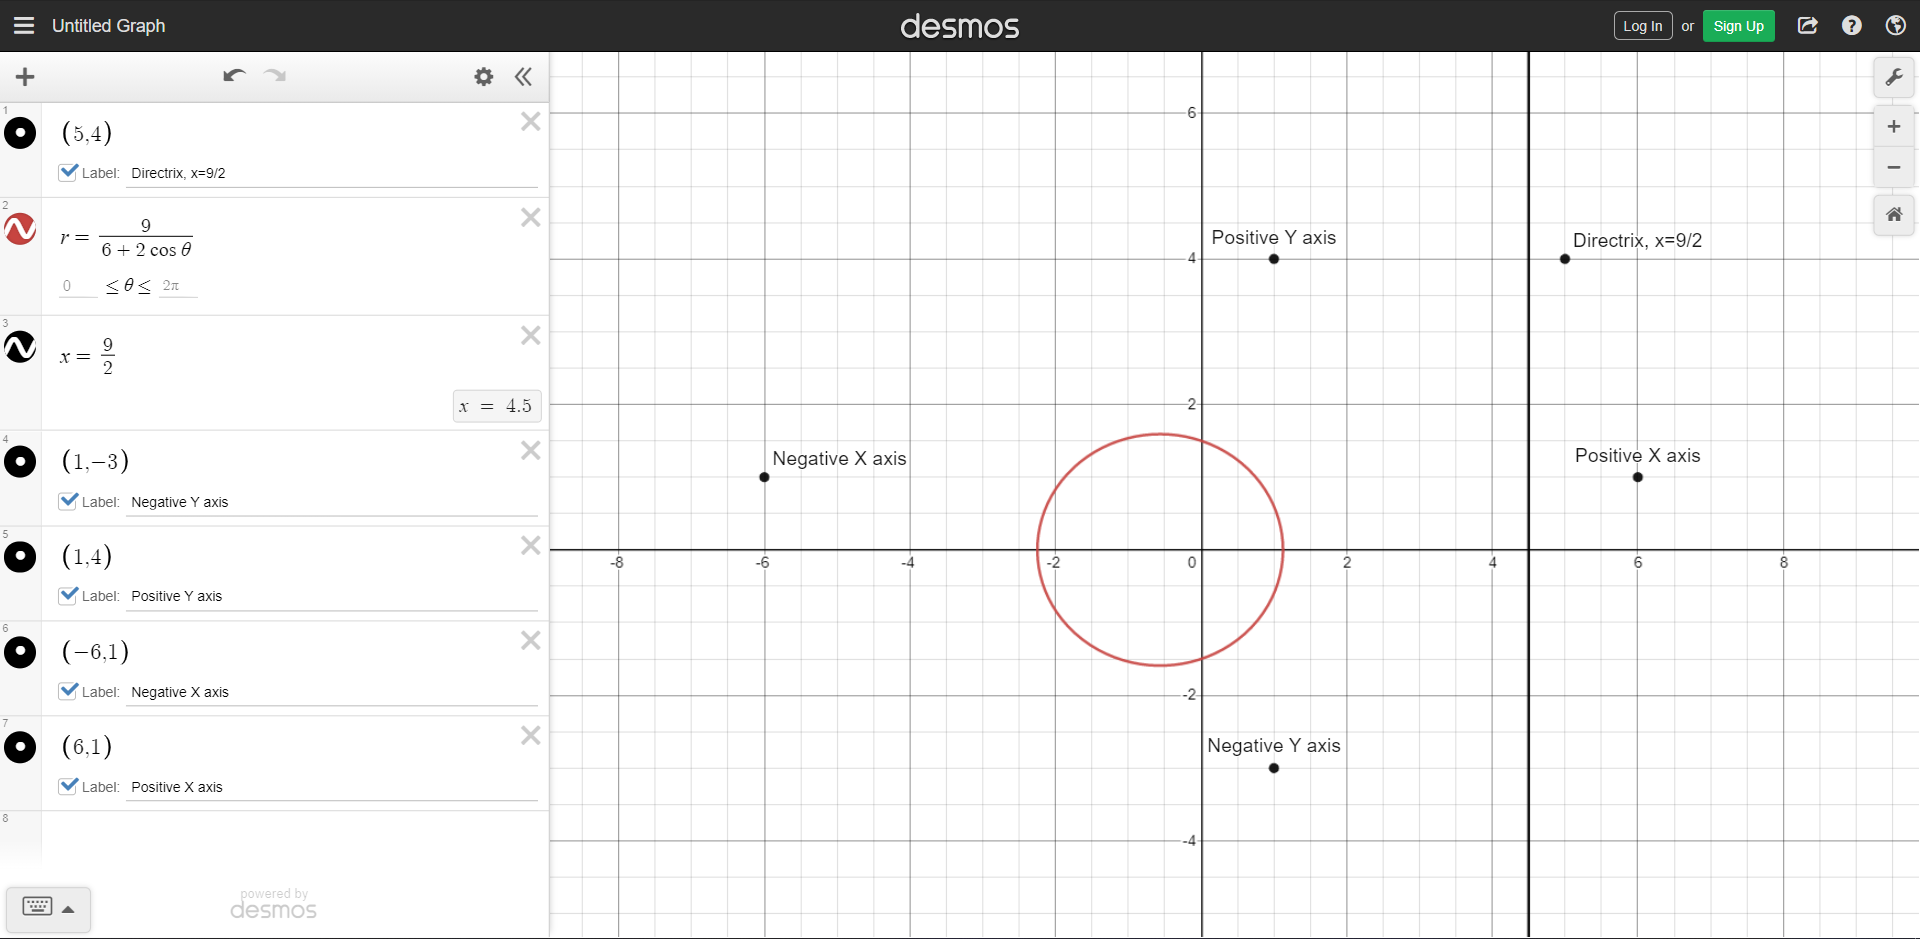
\includegraphics[width=15cm]{sketch question 4.PNG}
\end{newpage}
\begin{newpage}
    \begin{flushright}
    \textsc{Assignment 5}\\
    \textsc{Problem 5}\\
    [1 cm]
    \end{flushright}
\begin{center}
  \textbf{\Large \underline {Ans to the question no 05}}\\
  [0.5 cm]
\end{center}
\Large {Given, \\[3mm]
The cylindrical coordinates$ (r,\theta,z)=(\pi, \frac{\pi}{2},-2)$\\[3mm]
We know in terms of rectangular coordinates,\\[3mm]
$x=rcos\theta\\[3mm]
y=rsin\theta\\[3mm]
z=z\\[3mm]$
Here,\\[3mm]
$x=\pi cos\frac{\pi}{2}\\[3mm]
\Rightarrow x=\pi \cdot 0=0\\[3mm]$
Again,\\[3mm]
$y=\pi sin\frac{\pi}{2}\\[3mm]
\Rightarrow y=\pi \cdot 1\\[3mm]
\Rightarrow y=\pi =3.1416\\[3mm]$
And, $z=-2\\[5mm]
\therefore$ Rectangular coordinates $(x,y,z)=(0,3.1416,-2)\\[3mm]$}
\end{newpage}
\begin{newpage}
    \begin{flushright}
    \textsc{Assignment 5}\\
    \textsc{Problem 6}\\
    [1 cm]
    \end{flushright}
\begin{center}
  \textbf{\Large \underline {Ans to the question no 06}}\\
  [0.5 cm]
\end{center}
\Large {Given, \\[3mm]
The spherical coordinates$ (2,\theta,\phi)=(\frac{5\pi}{6}, \frac{\pi}{2},\pi)$\\[3mm]
We know in terms of rectangular coordinates,\\[3mm]
$x=e\cdot sin\phi cos\theta\\[3mm]
y=e\cdot sin\phi sin\theta\\[3mm]
z=e \cdot cos\phi\\[3mm]$
Here,\\[3mm]
$x=\frac{5\pi}{6} sin\pi cos\frac{\pi}{2}\\[3mm]
\Rightarrow x=\frac{5\pi}{6} \cdot 0\cdot 0=0\\[3mm]$
Again,\\[3mm]
$y=\frac{5\pi}{6}sin\pi sin\frac{\pi}{2}\\[3mm]
\Rightarrow y=\frac{5\pi} \cdot 0 \cdot 1=0\\[3mm]
And, z=\frac{5\pi}{6} cos\pi\\[3mm]
\Rightarrow z=-\frac{5\pi}{6}\\[3mm]
\Rightarrow z=-\frac{5\cdot 3.1416}{6}\\[3mm]
\Rightarrow z=-2.618\\[3mm]\\[3mm]
\therefore$ Rectangular coordinates $(x,y,z)=(0,0,-2.618)\\[3mm]$}
\end{newpage}
\end{document}